\chapter{Схема работы стандартного генетического алгоритма на бинарных строках}\label{StandardGA:section_shemebinaryGA}

В основу работы генетического алгоритма заложена имитация процесса эволюции живых организмов. Поэтому алгоритм представляет собой итерационный процесс (имитация смены поколений), работающий одновременно с несколькими взаимодействующими решениями (имитация популяции живых организмов).

Подробная схема, описывающая работу генетического алгоритма на бинарных строках ($ BinaryGeneticAlgorithm $), представлена ниже на рисунке.

\textbf{Замечание.} Довольно часто в литературе (например, \cite[с. 294]{book:Matveev2008}) рассматривается вариант, когда вначале отбираются потенциальные родители с помощью селекции (в «родительский пул»), а потом из них случайно отбираются родители для скрещивания. В данной модели генетического алгоритма это не происходит. Сразу после отбора двух родителей происходит скрещивание с целью получения одного потомка.

\begin{figure} [h] 
  \center
  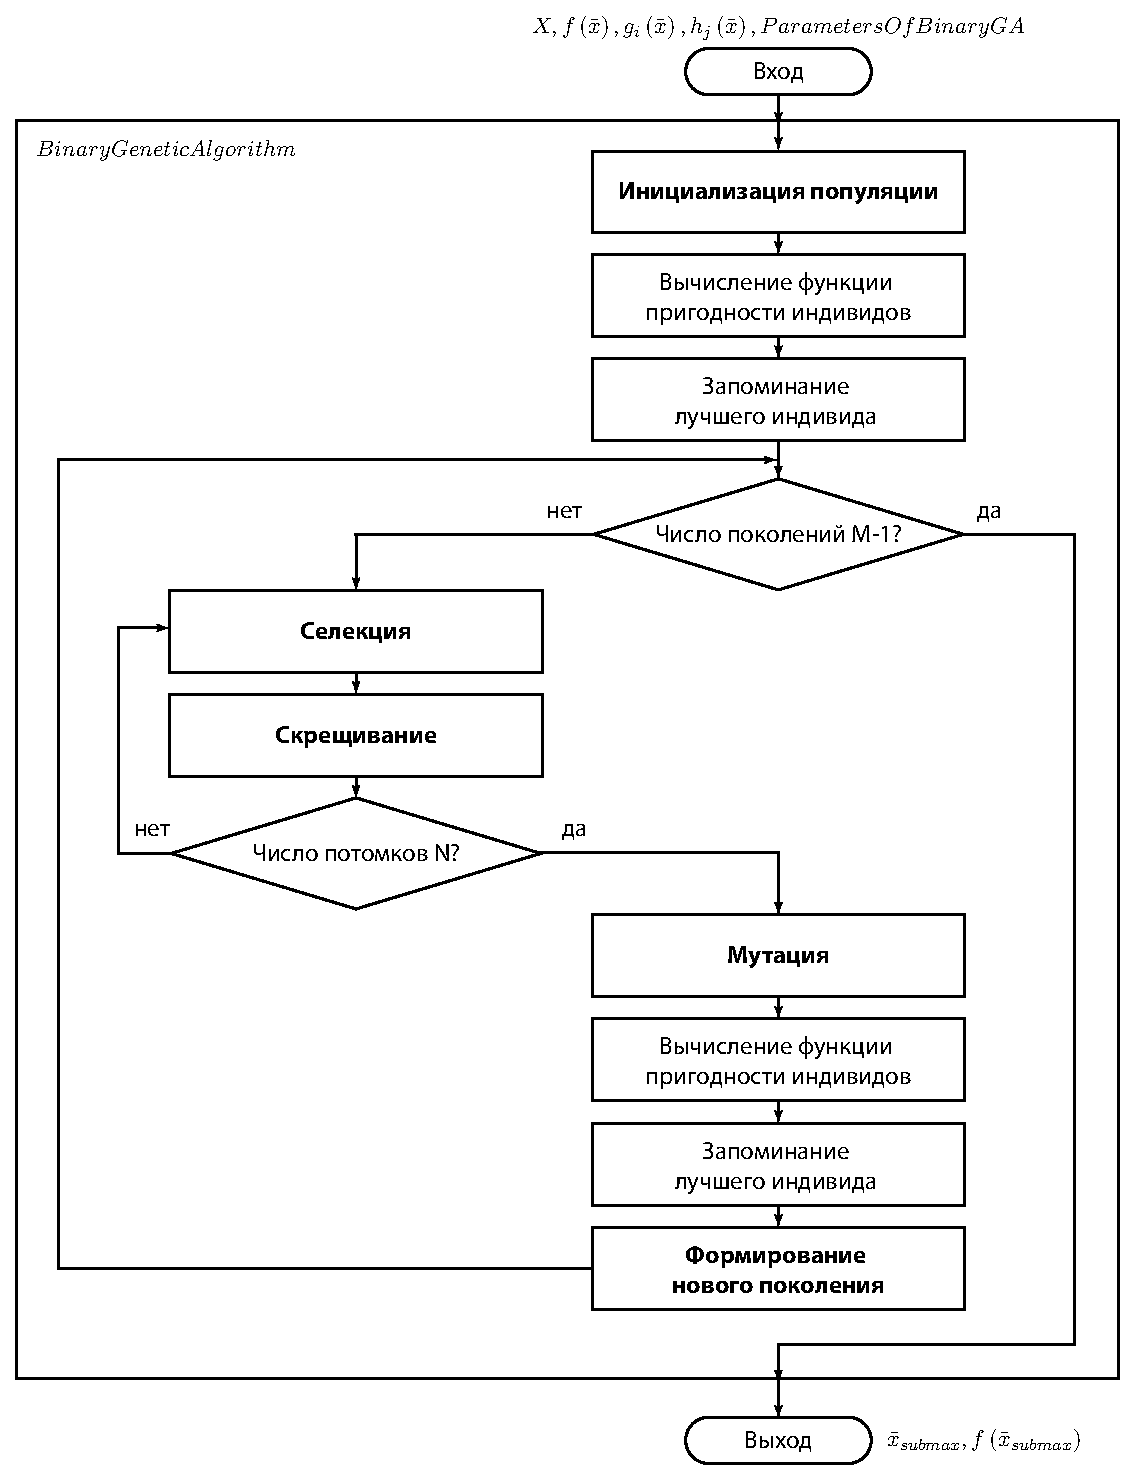
\includegraphics [scale=0.8] {GABinarySheme}
  \caption{Схема генетического алгоритма на бинарных строках} 
  \label{StandardGA:img:GABinarySheme}  
\end{figure}


\clearpage